\subsection{自旋波图像与海森堡模型}
对于自旋晶格系统的元激发,由于交换相互作用,系统的基态是磁有序状态,包括铁磁序,反铁磁序以及铁金氧磁序,相应的物理图像如图\ref{fig:ciyouxu}所示。
\begin{figure}
\begin{center}
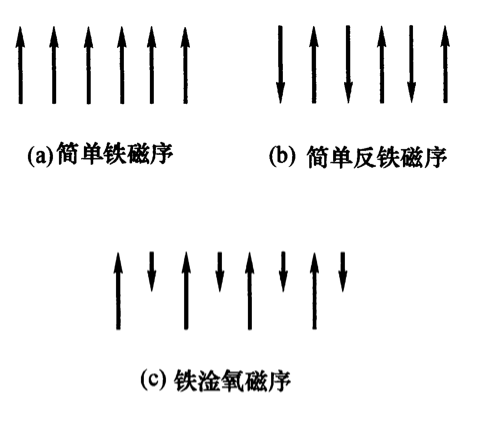
\includegraphics[height=8cm]{figures/ciyouxu.png}
\caption{三种常见的磁有序状态}
\label{fig:ciyouxu}
\end{center}
\end{figure}
自旋-自旋相互作用系统的哈密顿量通常可以表示为:
\[H=-\sum_{l,l'}'J_{l,l'}\hat{S}_l\cdot \hat{S}_{l'}\]
求和遍历所有的$l\neq l'$的空间格点处的自旋,这就是海森堡模型。\par
\subsection{铁磁自旋波理论}
对于铁磁体,交换积分J大于零。假设有N个自旋S的磁离子排成晶格。格点之间的自旋的对易关系为:
\[[S_l^i,S_{l'}^j]=i\epsilon^{i,j,k}S_l^k\delta_{l,l'}\]
一般采用$S^{\pm},S^z$作为独立变量,可以得到:
\[[S_l^{\pm},S_{l'}^z]=\mp S_l^{\pm}\delta_{l,l'}\]
\[[S_l^+,S_{l'}^-]=2S_{l}^z\delta{l,l'}\]
这时海森堡模型的系统哈密顿量可以写为:
\[H=-J\sum_{l,\delta}'\{S_l^zS_{l+\delta}^z+\frac{1}{2}(S_l^+S_{l+\delta}^-+S_l^-S_{l+\delta}^+)\}\]
这时系统的基态为:
\[\diracr{0}=\diracr{S}_1\diracr{S}_2\cdots \diracr{S}_N\]
其中$\diracr{S}_l$表示$\diracr{S,m=S}_l$
相应的基态能量为:
\[H\diracr{0}=-JNZS^2\diracr{0}\]
当第i个格点的自旋态发生偏转之后,比如说从基态的$\diracr{S,S}$偏转到$\diracr{S,S-1}$,由哈密顿量的形式可知,这个偏转将会逐渐传递到其他格点上,最后这个偏转逐渐平均到整个格点空间上。这说明格点间的交换作用使得单个格点上的自旋偏转以集体激发的形式表现。\par
为了刻画这个偏转的集体激发或是寻找系统的激发态,我们可以考虑一个量:
\[n=S-m\]
其中m为格点上自旋在z轴的投影的大小,n代表格点上与基态的偏转程度。与声子相似,用n标记自旋态,即:
\[\diracr{n}=\diracr{S,m}\]
那么可以得到:
\[S^+\diracr{n}=\sqrt{2S-(n-1)}\sqrt{n}\diracr{n-1}\]
\[S^-\diracr{n}=\sqrt{2S-n}\sqrt{n+1}\diracr{n+1}\]
对于这样的$\diracr{n}$态,引入常规的产生湮灭算符:
\[a\diracr{n}=\sqrt{n}\diracr{n-1}\]
\[a^+\diracr{n}=\sqrt{n+1}\diracr{n+1}\]
\[a^+a\diracr{n}=n\diracr{n}\]
从而可以得到算符之间的变换关系,称之为\textcolor{red}{霍斯坦因-普里马可夫变换}\par
\[\hat{S}^+=(\sqrt{2S-a^+a})a\]
\[\hat{S}^-=a^+(\sqrt{2S-a^+a})\]
\[\hat{S}^z=(S-a^+a)\]
利用$a,a^+$与利用$S^+,S^-,S^z$等具有等价的效益,他们俩彼此等价,利用$a,a^+$表示系统的哈密顿量为:
\[H=-J\sum'_{l,\delta} \{(S-a_l^+a_l)(S-a_{l+\delta}^+a_{l+\delta})+\frac{1}{2}\sqrt{2S-a_l^+a_l}a_la_{l+\delta}^+\sqrt{2S-a_{l+\delta}^+a_{l+\delta}}+\frac{1}{2}a_l^+\sqrt{2S-a_l^+a_l}\sqrt{2S-a_{l+\delta}^+a_{l+\delta}}a_{l+\delta}\}\]
算符之间的对易关系为:
\[[a_l,a_{l'}^+]=\delta_{l,l'}\]
由上面的表达是可知,由于根号项的存在使得问题的严格解很难求解,但如果磁的自旋偏离基态较少,可以把根号展开,这便是低温时的近似解。\par
低温近似下,作近似$\sqrt{2S-a^+a}\rightarrow \sqrt{2S}$,并且忽略掉算符的四次方项,那么可以得到哈密顿量(这时哈密顿量呈现出二次型的形式):
\[H_0=-NZJS^2+2ZJS\sum_la_l^+a_l-JS\sum_{l,\delta}'(a_la_{l+\delta}^++a_l^+a_{l+\delta})\]
其中第一项为基态能量,第二项代表第l个格点上自旋的偏转带来的能量,第三项代表不同格点之间的耦合。\par
为了讲这个二次型对角化,需要对算符作正则变换:
\[a_l=\frac{1}{\sqrt{N}}\sum_k e^{ikl}b_k\]
\[a_l^+=\frac{1}{\sqrt{N}}\sum_k e^{-ikl}b_k^+\]
利用傅立叶变换的反演可以给出逆变换。这时系统的哈密顿量为:
\begin{align*}
\notag H_0&=-NZJS^2+2ZJS\sum_lb_l^+b_l-ZJS\sum_k\gamma_k(b_k^+b_k+b_kb_k^+)\\
&=E_0+\sum_k\hbar\omega_k(b_k^+b_k)
\end{align*}
其中$\gamma_k$为结构因子:
\[\gamma_k=Z^{-1}\sum_{\delta}e^{ik\delta}=\gamma_{-k}\]
$\omega_k$为自旋波频率:
\[\hbar\omega_k=2ZJS(1-\gamma_k)\]
从而整个系统都已经变为对角化的形式,能直接求解。\par

\subsection{铁磁体的低温磁化强度}